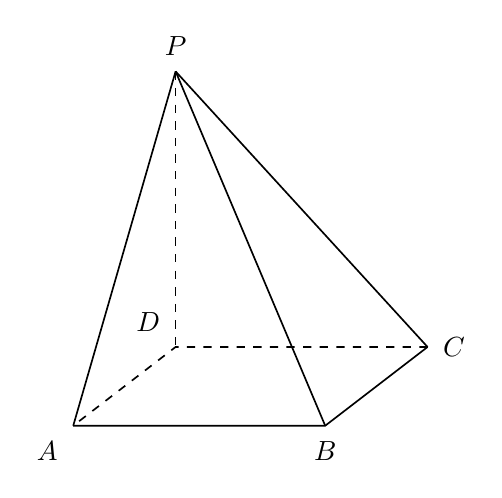
\begin{tikzpicture}[x=1cm,y=1cm,font=\normalsize,line width=.6pt]
\coordinate (P) at (1.3000000000,5.0000000000);
\coordinate (D) at (1.3000000000,1.5000000000);
\coordinate (A) at (0,0.5);
\coordinate (B) at (3.2,0.5);
\coordinate (C) at (4.5,1.5);
% base
\draw[solid] (A) -- (B) -- (C);
\draw[dashed] (C) -- (D) -- (A);
% lateral edges
\draw[solid] (P) -- (A);
\draw[solid] (P) -- (B);
\draw[solid] (P) -- (C);
\draw[dashed] (P) -- (D);
\node[above,yshift=2pt] at (P) {$P$};
\node[above left=2pt] at (D) {$D$};
\node[below left,xshift=-2pt,yshift=-2pt] at (A) {$A$};
\node[below,yshift=-2pt] at (B) {$B$};
\node[right,xshift=2pt] at (C) {$C$};
\end{tikzpicture}
